\needspace{9\baselineskip}
\section{Hallway relaxations}\label{sec:relaxations}

\subsection{Rotated hallways}

For an angle $a\in\R$ let
\[
f_a(x,y)=x\cos a+y\sin a, \qquad g_a(x,y)=-x\sin a+y\cos a
\]
be the coordinates in a frame rotated by $a$, so that $R_{-a}z=(f_a(z),g_a(z))$. For $\bu=(u_1,u_2)\in\R^2$ we define the rotated and translated hallway
\begin{equation}\label{eq:La}
\begin{split}
L_a(\bu)&=R_a(\bu+L_0)\\
&=\{u_1\le f_a\le u_1+1,\ g_a\le u_2+1\}\cup\{f_a\le u_1+1,\ u_2\le g_a\le u_2+1\}.
\end{split}
\end{equation}
This is the notation of \cite{kallusromik2018}, except that $a$ may be any real angle, not only one between $0\dg$ and $90\dg$. We call the two sets in \eqref{eq:La} the \emph{arms} of the hallway: the first is the image of $\Lv$, the arm that leaves the corner, and the second the image of $\Lh$, the arm that leads into it. We also use the mirrored hallways $\rho(L_b(\bv))$; see \cref{fig:hallways}.

The next lemma describes the hallway in the frame of the sofa. In part~(ii) the mirrored hallway appears with the opposite angle, because $\rho$ reverses the sense of rotation: $\rho\circ R_\theta\circ\rho^{-1}$ is a rotation by $-\theta$ followed by a translation.

\needspace{5\baselineskip}
\begin{lem}[The hallway seen from the sofa]\label{lem:frame}
Let $S\subset\R^2$ and let $\Psi(z)=R_\theta z+\mathbf{x}$ be a rigid motion.
\begin{enumerate}[label=(\roman*)]
\item If $\Psi(S)\subset L_0$, then $S\subset L_{-\theta}(\bu)$ for some $\bu\in\R^2$.
\item If $\Psi(S)\subset\rho(L_0)$, then $S\subset\rho(L_{\theta}(\bv))$ for some $\bv\in\R^2$.
\item If $\Psi(S)\subset R_{90\dg}L_0+\mathbf{q}$ for some $\mathbf{q}\in\R^2$, then $S\subset L_{90\dg-\theta}(\bu)$ for some $\bu\in\R^2$.
\end{enumerate}
\end{lem}

\begin{proof}
In each case $S\subset \Psi^{-1}(Y)=R_{-\theta}(Y-\mathbf{x})$, where $Y$ is the hallway in question. For (i), $R_{-\theta}(L_0-\mathbf{x})=L_{-\theta}(-\mathbf{x})$.

\needspace{9\baselineskip}
For (ii), separate the reflection $\rho$ into its linear part and a translation: $\rho(z)=\sigma z+e_2$, where $\sigma(x,y)=(x,-y)$ and $e_2=(0,1)$. Put $\mathbf{w}=\sigma(e_2-\mathbf{x})$, so that $\rho(L_0)-\mathbf{x}=\sigma(L_0+\mathbf{w})$. Using $R_{-\theta}\sigma=\sigma R_\theta$, we get
\begin{align*}
R_{-\theta}\big(\rho(L_0)-\mathbf{x}\big)&=\sigma R_\theta(L_0+\mathbf{w})=\sigma\big(L_\theta(\mathbf{w})\big)=\rho\big(L_\theta(\mathbf{w})\big)-e_2\\
&=\rho\big(L_\theta(\mathbf{w})+e_2\big)=\rho\big(L_\theta(\mathbf{w}+R_{-\theta}e_2)\big).
\end{align*}
In the second line we used that $\rho(Y)-e_2=\rho(Y+e_2)$ for every set $Y$, and that $R_\theta(L_0+\mathbf{w})+e_2=R_\theta(L_0+\mathbf{w}+R_{-\theta}e_2)$. Hence $S\subset\rho\big(L_\theta(\bv)\big)$ with $\bv=\mathbf{w}+R_{-\theta}e_2$.

For (iii), $R_{-\theta}(R_{90\dg}L_0+\mathbf{q}-\mathbf{x})=R_{90\dg-\theta}\big(L_0+R_{-90\dg}(\mathbf{q}-\mathbf{x})\big)=L_{90\dg-\theta}\big(R_{-90\dg}(\mathbf{q}-\mathbf{x})\big)$.
\end{proof}

Thus a sofa that has rotated clockwise by $a$ during a right turn (so $\theta=-a$) lies in a hallway $L_a(\bu)$, and one that has rotated counterclockwise by $b$ during a left turn lies in a mirrored hallway $\rho(L_b(\bv))$. Romik's shape rotates monotonically by $90\dg$ in both turns, so for it these angles fill $[0\dg,90\dg]$. A general motion need not reach them all; \cref{sec:reduction} shows which ones every sofa of large area must reach.


\needspace{8\baselineskip}
\begin{figure}[h]
\centering
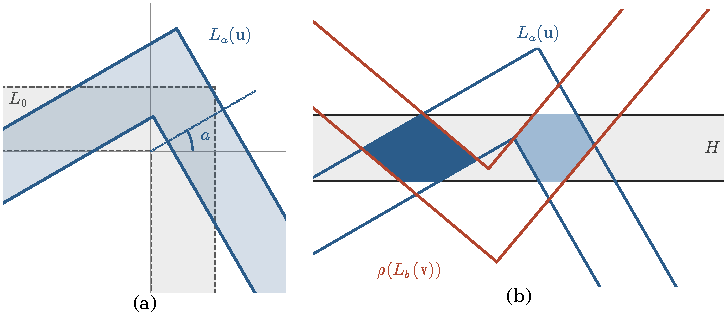
\includegraphics[width=0.9\textwidth]{figures/fig_hallways.pdf}
\caption{(a) The hallway $L_0$ (dashed) and the rotated and translated hallway $L_a(\bu)$ for $a=30\dg$. (b) A hallway $L_a(\bu)$ with $a=30\dg$ and a mirrored hallway $\rho(L_b(\bv))$ with $b=40\dg$. Their intersection with the strip $H$ has two connected components, of areas $1.005$ (dark) and $0.859$ (light); the value of $\lamstar$ is the larger one.}
\label{fig:hallways}
\end{figure}

\subsection{The relaxation}

\begin{defn}\label{def:G}
For finite sets $A,B\subset\R$ of angles let
\begin{equation}\label{eq:G}
G(A;B)=\sup\,\lamstar\Big(H\cap\bigcap_{a\in A}L_a(\bu_a)\cap\bigcap_{b\in B}\rho\big(L_b(\bv_b)\big)\Big),
\end{equation}
where the supremum is over all choices of vectors $\bu_a,\bv_b\in\R^2$.
\end{defn}

When $B=\emptyset$ and $A\subset(0\dg,90\dg)$, this is the quantity $G_{\boldsymbol\alpha}$ of Kallus and Romik \cite{kallusromik2018}. The sets $A$ and $B$ correspond to the right turn and the left turn.

\begin{lem}\label{lem:relax}
Let $S\subset H$ be closed and connected. If $S\subset L_a(\bu_a)$ for every $a\in A$ and $S\subset\rho(L_b(\bv_b))$ for every $b\in B$, then $\lambda(S)\le G(A;B)$.
\end{lem}

\begin{proof}
$S$ is a connected subset of the intersection in \eqref{eq:G}, so it lies in a single connected component of it.
\end{proof}

We also need two simple estimates. The first underlies the angle conditions in \cref{sec:reduction}.

\begin{lem}[Two strips]\label{lem:strips}
Let $S\subset H$ be measurable and let $\Psi(z)=R_\theta z+\mathbf{x}$ be a rigid motion.
\begin{enumerate}[label=(\roman*)]
\item If $\Psi(S)\subset V$, then $\lambda(S)\le 1/|\cos\theta|$.
\item If $\Psi(S)$ lies in a horizontal strip $\R\times[c,c+1]$, then $\lambda(S)\le1/|\sin\theta|$.
\end{enumerate}
Here $1/0=\infty$.
\end{lem}

\begin{proof}
In case (i), $S$ lies in the intersection of $H$ with the strip $\Psi^{-1}(V)$, also of width $1$, whose direction makes an angle of $90\dg-\theta$ with the horizontal. Two strips of width $1$ whose directions make an angle $\varphi$ with $\sin\varphi\neq0$ intersect in a parallelogram of area $1/|\sin\varphi|$. For $\varphi=90\dg-\theta$ we have $|\sin\varphi|=|\cos\theta|$, and if $\cos\theta=0$ there is nothing to prove. Case (ii) is the same with the angle $-\theta$.
\end{proof}

\needspace{8\baselineskip}
The second estimate bounds the length of a connected set that fits in a rotated hallway and in $H$.

\begin{lem}[Width]\label{lem:width}
Let $0\dg<a<90\dg$, write $c=\cos a$ and $s=\sin a$, and let
\[
W_a=\frac{1+s}{c}+\frac{1+c}{s}.
\]
If $K$ is a connected subset of $H\cap L_a(\bu)$ or of $H\cap\rho(L_a(\bu))$, then the projection of $K$ to the $x$-axis is an interval of length at most $W_a$. Consequently $\diam K\le\sqrt{W_a^2+1}$.
\end{lem}

\begin{proof}
Since $\rho$ preserves $H$ and $x$-coordinates, it suffices to treat $L_a(\bu)$. Let $0\le y\le1$. A point $(x,y)$ of the first arm satisfies $u_1\le xc+ys\le u_1+1$, so $x$ lies in the interval $[(u_1-s)/c,\,(u_1+1)/c]$ of length $(1+s)/c$. A point of the second arm satisfies $u_2\le -xs+yc\le u_2+1$, so $x$ lies in $[(-u_2-1)/s,\,(c-u_2)/s]$, of length $(1+c)/s$. The projection of $K$ is connected, hence an interval, and it is contained in the union of these two intervals; so its length is at most the sum of their lengths.
\end{proof}

For example, $W_{45\dg}=2+2\sqrt2$, and $W_a=5$ for $a=\arcsin(3/5)$ and $a=\arcsin(4/5)$.

\subsection{Hallways at \texorpdfstring{$45\dg$}{45 degrees}}\label{sec:45}

We need two facts about hallways rotated by odd multiples of $45\dg$: \cref{lem:sideways}, which is used for both theorems, and \cref{prop:onehalf}, which gives \cref{thm:hand}. We say that the corner of $L_0$ points in the direction $45\dg$, the direction of the vector from its inner corner $(0,0)$ to its outer corner $(1,1)$. Hence the corner of $L_a(\bu)$ points in the direction $a+45\dg$, and that of $\rho(L_b(\bv))$ in the direction $-(b+45\dg)$. The first fact concerns the four cases in which the corner points horizontally, so that the hallway lies ``sideways'' across $H$ (\cref{fig:45}(a)).

\begin{figure}[h]
\centering
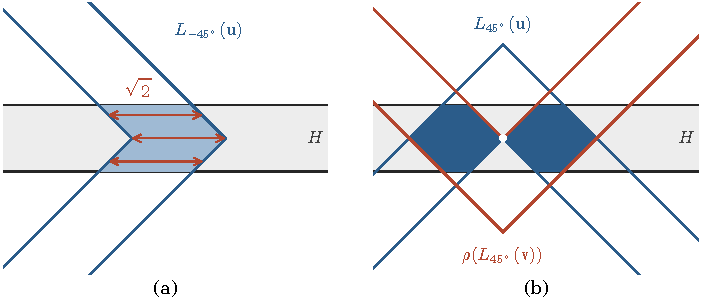
\includegraphics[width=\textwidth]{figures/fig_45.pdf}
\caption{Hallways at $45\dg$. (a) A sideways hallway $L_{-45\dg}(\bu)$. Every horizontal line meets it in a segment of length $\sqrt2$, so it meets $H$ in area exactly $\sqrt2$ (\cref{lem:sideways}). (b) The extremal configuration of \cref{prop:onehalf}: for $\bu=\bv=(0,1/\sqrt2)$ the set $H\cap L_{45\dg}(\bu)\cap\rho(L_{45\dg}(\bv))$ consists of two squares of side $1$, each cut off by $H$, which touch at the point $(-\tfrac12,\tfrac12)$. Its area is $2\sqrt2-1$.}
\label{fig:45}
\end{figure}


\needspace{7\baselineskip}
\begin{lem}[Sideways hallways]\label{lem:sideways}
Let $X$ be one of $L_{-45\dg}(\bu)$, $L_{135\dg}(\bu)$, $\rho(L_{-45\dg}(\bu))$ and $\rho(L_{135\dg}(\bu))$, for some $\bu\in\R^2$. Then every horizontal line meets $X$ in a segment of length exactly $\sqrt2$. Consequently $\lambda(H\cap X)=\sqrt2$, and every measurable set $S\subset H\cap X$ has $\lambda(S)\le\sqrt2$.
\end{lem}

\begin{proof}
First let $X=L_{-45\dg}(\bu)$. Then $f=(x-y)/\sqrt2$ and $g=(x+y)/\sqrt2$, and by \eqref{eq:La}
\[
X=\{f\le u_1+1,\ g\le u_2+1\}\setminus\{f<u_1,\ g<u_2\}.
\]
On the horizontal line at height $y$, both $f$ and $g$ increase with $x$ at rate $1/\sqrt2$. Put $\xi_1=\sqrt2\,u_1+y$ and $\xi_2=\sqrt2\,u_2-y$. The first set above meets the line in the points with $x\le\min(\xi_1,\xi_2)+\sqrt2$, and the removed set in the points with $x<\min(\xi_1,\xi_2)$. So the line meets $X$ in the segment $x_0\le x\le x_0+\sqrt2$ with $x_0=\min(\xi_1,\xi_2)$.

The other three cases follow, because $L_{135\dg}(\bu)=R_{180\dg}L_{-45\dg}(\bu)$ and both the rotation $R_{180\dg}$ and the reflection $\rho$ map horizontal lines to horizontal lines without changing lengths. Integrating the length $\sqrt2$ over $0\le y\le1$ gives $\lambda(H\cap X)=\sqrt2$.
\end{proof}

The second fact is that the relaxation with one angle, $45\dg$, on each side can be computed exactly.

\begin{prop}[One angle on each side]\label{prop:onehalf}
For all $\bu,\bv\in\R^2$,
\[
\lambda\big(H\cap L_{45\dg}(\bu)\cap\rho(L_{45\dg}(\bv))\big)\le 2\sqrt2-1,
\]
with equality when $\bu=\bv=(0,1/\sqrt2)$, in which case the set is connected. In particular $G(\{45\dg\};\{45\dg\})=2\sqrt2-1$.
\end{prop}

The proof, an exact computation of areas by slicing along horizontal lines, is in \cref{app:onehalf}. For comparison, with the hallway $L_{45\dg}(\bu)$ alone the supremum of $\lamstar$ is $2\sqrt2$: this is Hammersley's bound, written in the language of relaxations \cite[Section~2]{kallusromik2018}, and it comes from the two arms of $L_{45\dg}(\bu)$, each of which meets $H$ inside a parallelogram of area $\sqrt2$. \Cref{fig:45}(b) shows the effect of the mirrored hallway in the extremal configuration: it cuts each arm down to a unit square. A unit square tilted by $45\dg$ meets $H$ in area at most $\sqrt2-\tfrac12$, and both squares attain this, so the total is $2\sqrt2-1$, exactly $1$ less than Hammersley's bound.
